\documentclass{../template/texnote}

\title{\textbf{Transforming the landscape of ML using Transformers}}[author={Linn Abraham}]

\begin{document}
    \maketitle \currentdoc{note}
    %<*note>

\section{Introduction}
By now you must have heard about ``Transformers'' at least once. I am not talking about the movie franchise, but the machine learning model that forms part of the Chat-GPT acronym. 
If you don't know, GPT stands for Generative Pre-trained Transformer. 
In this article, I aim to build the case for transformers. How they revolutionized, not only the field of Natural Language Processing (NLP) but the whole machine learning landscape.
One of the goals is to give you an intuition of what ``attention'' blocks in Transformers actually achieve.
Through this I hope you also get an intuition for how technologies like Chat-GPT are stretching the boundaries of what AI can currently achieve.

\section{The Role of Auto-Encoders}
A key idea that has enabled this sudden rise of capability is a class of ML models called auto-encoders.
The advantage they bring to the table is that, they are a kind of unsupervised ML technique. 
Meaning that they do not require each training sample to be associated with a ``label'' that then becomes the ground truth for teaching the machine.
This is because auto-encoders are designed to learn a model that can reproduce the input as the output.
Think of a CNN which tries to learn how to accurately generate the input image in the output.
Each pixel of the input image itself then becomes the label for that pixel.
Such architectures have two parts - an encoder which forms a bottleneck by distilling the input image into a lower dimensional space.
And a decoder that tries to generate the final output from the output of the encoder.
If trained successfully, we expect the weights of the network to store information about the underlying process that generated the input data.
In the context of an NLP model, the input can be a sentence and the output can be predicting each subsequent word from the one preceding it.
The fact that auto-encoders can learn from unlabelled data has a huge implication, it saves machine learning engineers from spending countless hours preparing labelled data.
Instead, since the internet is mostly a huge corpus of text, they have at their disposal a gold mine of training data for training the machine.
The only deciding factor now would be who has the most resources to train networks on such huge datasets.

\section{Does Chat-GPT really understand human language?}
Chat-GPT is a product of research in Natural Language Processing (NLP), a subdomain of Artificial Intelligence.
The terminology ``Natural Language'' comes because there exists ``programming languages'' that are man-made languages designed for humans to communicate with machines.
Let's look at some of the tasks that NLP models are trained to perform: 
\begin{itemize}

\item Classifying whether a movie review is positive or negative - this is called sentiment analysis.
\item Summarizing a news article in a few words - text summarization.
\item Translating a sentence from English to French - machine translation.
\item What should be the next word in this (incomplete) sentence? - text generation%language modelling.
%Sentiment Analysis - An example can be identifying whether a movie review is positive or negative. 
%The usual tasks that NLP models are trained to excel are the following:

\end{itemize}
Chat-GPT itself is called a Large Language Model or LLM for short. 
Although, today LLMs are capable of much more, it is helpful to focus on one of their abilities - text generation.
Let's think of Chat-GPT and similar chatbots as systems that can predict the next word given a seed word or sentence.
Once we have a system that can do this, if the output along with the initial prompt is fed back to the input we can generate the next word in the sequence.
So this is what basically happens under-the-hood of Chat-GPT.
But to make it possible to do all those amazing things you have seen it do - it leverages the power of the ``transformer" network together with the capacity of learning 
150 billion model parameters.


\section{Understanding Transformers}
Before transformers, the dominant algorithms were LSTMs and GRUs which were modifications of something called a Recurrent Neural Network (RNN).
These were notoriously difficult to train, especially on large datasets because of the sequential nature of their algorithms.
Which obviously meant they could not take advantage of the huge parallelization abilities of modern GPUs.
One of the contribution of the original paper, that introduced the transformers, was the ``Attention'' block which helped alleviate this problem.
The way they solved the problem is by introducing an ``attention'' block that once trained can produce outputs in parallel for each token in an input sentence.
%that produces one output for each input token in the sentence.
%This output can be thought of as a score that gives how much attention it receives from the rest of the tokens in the sentence.

To understand transformers we need to recognize what they were designed for. 
The transformer architecture was designed for machine translation tasks.
In the terminology of NLP, it is a kind of sequence-to-sequence model.
It employs the auto-encoder algorithm that we had talked about earlier.
But instead of using LSTMs or such for the encoder-decoder part it uses ``attention'' blocks and MLPs along with the usual mix of residual connections and normalization layers (see Fig. \ref{fig:encoder}).
\begin{figure}
    \centering
    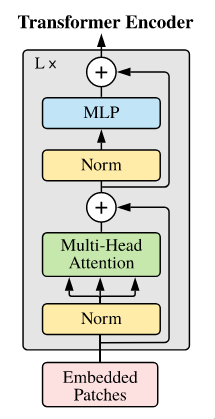
\includegraphics{Linn/transformer_encoder.png}
    \caption{A sketch of the transformer encoder block. Image Credit:Dosovitskiy et. al.}
    \label{fig:encoder}
\end{figure}
In the process of learning to reproduce the input, auto-encoders learn a hidden representation of the input (feature) space, which is called the embedding (vector).
Thus the transformer encoder after being trained has learnt some useful representation from the input language.
Which it then uses to do the reverse, convert the embeddings back to a sentence, this time to another language.
%This is a tad different from the way it is used in text generators to generate the next word in the same language.
At the least, it is helpful to learn how this transformer encoder works since the encoder can be used for other tasks such as text classification etc.

\section{The Attention Block}
What made existing models slow, before Transformers came into the picture, was the sequential process of processing each input token in a sentence and updating 
a state variable. You can think of this state variable as the memory of a neural network. 
The transformer bypasses the need to do sequential computations with the ``Attention'' block, which you can think of as a smaller neural network that learns three weight matrices from the data, which we call
Query(Q), Value(V) and Key(K) for reasons that might become clear later on.
The Query matrix multiplied by the transpose of the Key matrix produces a score matrix where each element shows how much a word (token) should pay attention to another word (token).
You can think of the word ``attention'' as asking the following question for each word in a sentence - 
Which other words in this sentence are important for understanding this word? 
That is,  how related each word is to every other word.
The key insight here is that, despite the fact that the Attention mechanism computes an attention score for each pair of tokens in a sentence, it achieves parallelization through the use of
matrix operations.
%The actual transformer model employs something called ``multi-head attention'' 

We can build on this intuition in a future article which would try to understand how the ``multi-head attention'' block is different from what we just learnt.
Also it would explore the other components like MLP layers that together complete the transformer encoder block.
%\cite{cholletDeepLearningPython2021}
%\cite{vaswaniAttentionAllYou}
\cite{dosovitskiyIMAGEWORTH16X162021}
\begin{thebibliography}{2}
\providecommand{\natexlab}[1]{#1}
\providecommand{\url}[1]{\texttt{#1}}
\expandafter\ifx\csname urlstyle\endcsname\relax
  \providecommand{\doi}[1]{doi: #1}\else
  \providecommand{\doi}{doi: \begingroup \urlstyle{rm}\Url}\fi

\bibitem[Chollet(2021)]{cholletDeepLearningPython2021}
Fran{\c c}ois Chollet.
\newblock \emph{Deep Learning with {{Python}}}.
\newblock Manning, Shelter Island, NY, second edition edition, 2021.
\newblock ISBN 978-1-61729-686-4.

\bibitem[Vaswani et~al.()Vaswani, Shazeer, Parmar, Uszkoreit, Jones, Gomez,
  Kaiser, and Polosukhin]{vaswaniAttentionAllYou}
Ashish Vaswani, Noam Shazeer, Niki Parmar, Jakob Uszkoreit, Llion Jones,
  Aidan~N Gomez, {\L}ukasz Kaiser, and Illia Polosukhin.
\newblock Attention is {{All}} you {{Need}}.

\bibitem[Dosovitskiy et~al.(2021)Dosovitskiy, Beyer, Kolesnikov, Weissenborn,
  Zhai, Unterthiner, Dehghani, Minderer, Heigold, Gelly, Uszkoreit, and
  Houlsby]{dosovitskiyIMAGEWORTH16X162021}
Alexey Dosovitskiy, Lucas Beyer, Alexander Kolesnikov, Dirk Weissenborn,
  Xiaohua Zhai, Thomas Unterthiner, Mostafa Dehghani, Matthias Minderer, Georg
  Heigold, Sylvain Gelly, Jakob Uszkoreit, and Neil Houlsby.
\newblock {{AN IMAGE IS WORTH 16X16 WORDS}}: {{TRANSFORMERS FOR IMAGE
  RECOGNITION AT SCALE}}.
\newblock 2021.

\end{thebibliography}

\vspace{0.5cm}
\noindent\fbox{%
	\parbox{\textwidth}{%
		\textbf{About the Author}\vspace{0.2cm} \\
		\textbf{Linn Abraham} is a researcher in Physics, specializing in A.I. applications to astronomy. 
He is currently involved in the development of CNN based Computer Vision tools for
prediction of solar flares from images of the Sun, morphological classifications of galaxies from optical images surveys and radio galaxy source extraction from radio observations.
	}
}
    %</note>
    \printbibliography
\end{document}
